\section{Current Results}\label{s:current_results}

\begin{table}[htbp]
    \centering
    \caption{Status of current results.}\label{table:current_results}
    \begin{tabular}{lp{0.25\textwidth}p{0.4\textwidth}}
        \toprule
        Name                      & Status & Physics \\
        \midrule
        Simple Box                &        &         \\
        Wave                      &        &         \\
        Simple ShearBand          &        &         \\
        Sandia Fracture Challenge &        &         \\
        Tophat                    &        &         \\
        Torsion                   &        &         \\
        \bottomrule
    \end{tabular}
\end{table}

\FloatBarrier{}

\subsection{Simple Box}\label{ss:simple_box}

\subsection{Wave}\label{ss:wave}

\subsection{Simple ShearBand}\label{ss:simple_shearband}

The simple shear band problem consists of a box mesh put into pure shear. Periodic boundary conditions exist at $x=0$ and $x=0$ for $u_x$ and $u_y$.

The remeshing is set up so that the grid structure of the original mesh is preserved, with the same number of elements in the $x$ and $y$ directions, shown in Figure~\ref{fig:mesh_ex}. Final effective plastic strain and temperature fields are shown in Figure~\ref{fig:field_ex}.

\begin{figure}
    \begin{subfigure}{0.45\textwidth}
        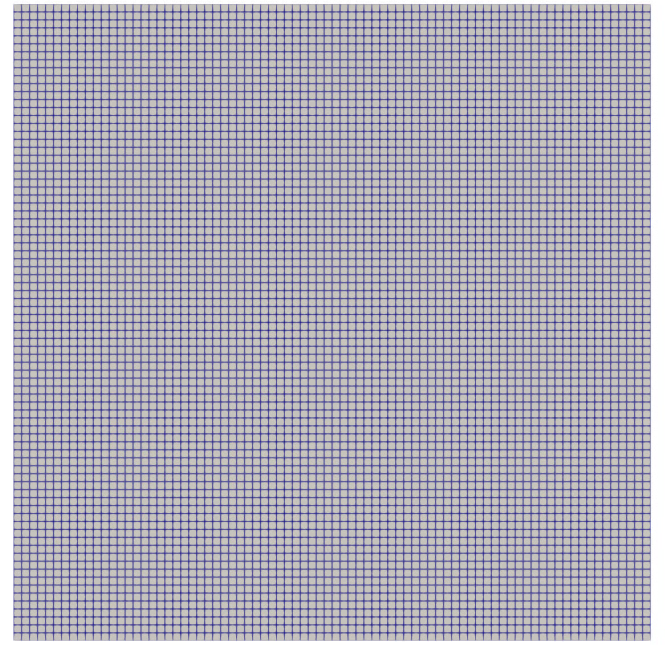
\includegraphics[width=0.8\textwidth]{results/pictures/simpleshearband/mesh0.png}    
    \end{subfigure}
    \begin{subfigure}{0.45\textwidth}    
        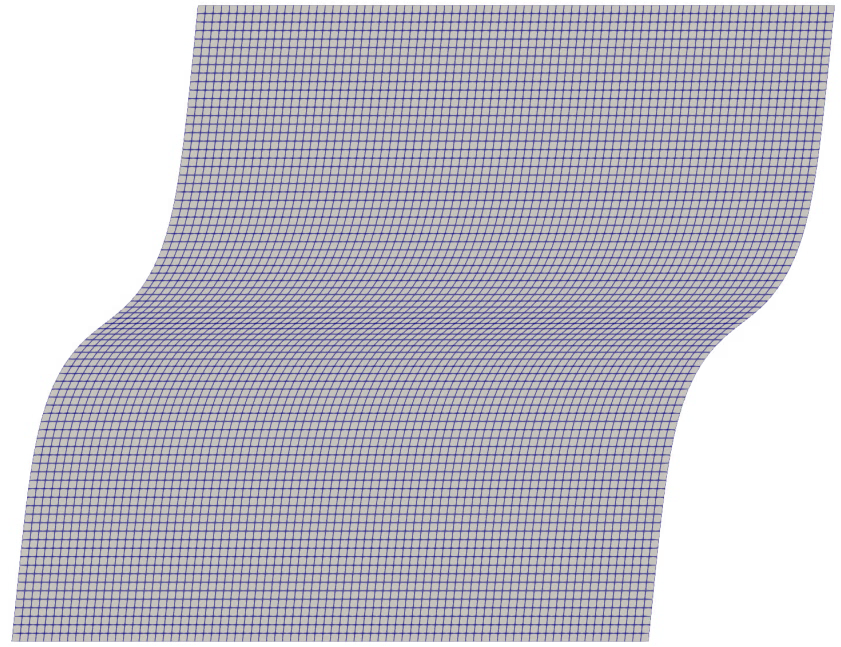
\includegraphics[width=\textwidth]{results/pictures/simpleshearband/mesh1.png}    
    \end{subfigure}
    \caption{Original and final mesh}\label{fig:mesh_ex}
\end{figure}


\begin{figure}
    \begin{subfigure}{0.45\textwidth}
        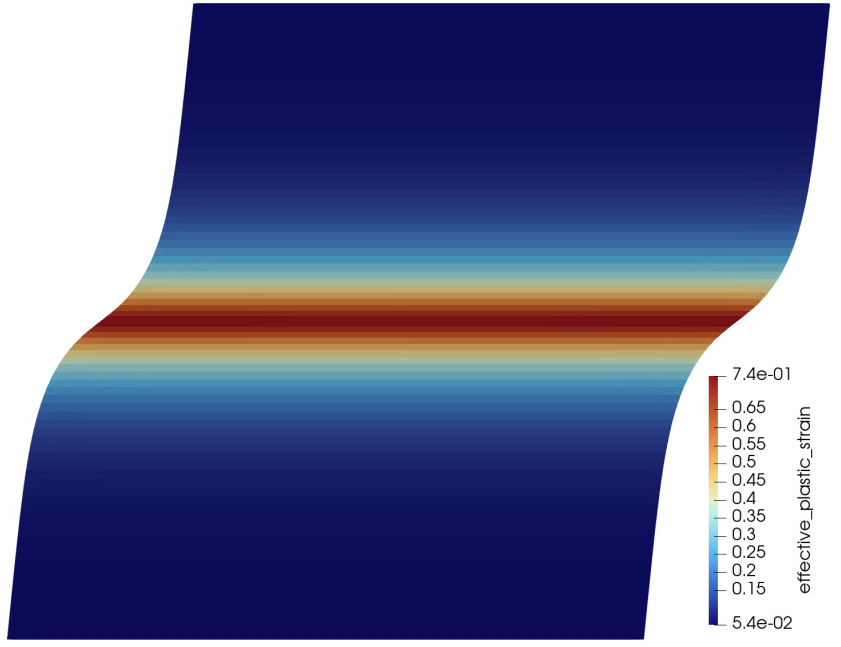
\includegraphics[width=\textwidth]{results/pictures/simpleshearband/ep_example.png}    
    \end{subfigure}
    \begin{subfigure}{0.45\textwidth}    
        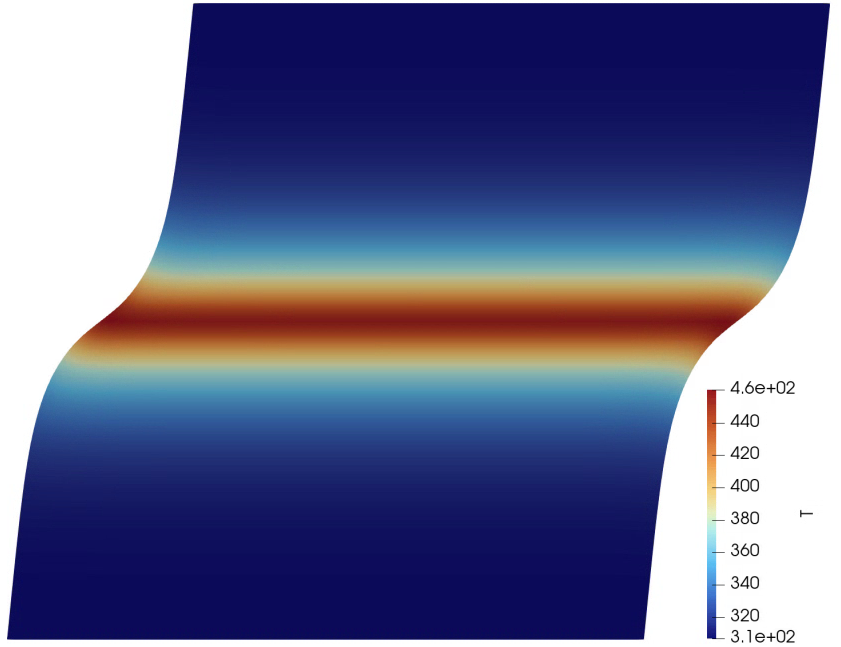
\includegraphics[width=\textwidth]{results/pictures/simpleshearband/T_example.png}    
    \end{subfigure}
    \caption{Final effective plastic strain~(left) and temperature fields~(right)}\label{fig:field_ex}
\end{figure}

% Global CSVs have quoted headers, so columns are referenced by index: 0 Time, 1 kinetic_energy_int, 2 psie_active_int, 3 total_energy.
% The first row of run1_global.csv is an all-zero placeholder at the restart time, so it is dropped.
% The zoomed panel puts kinetic (solid, left axis) and elastic (dashed, right axis) energy on separate y axes;
% it has no legend of its own and shares the line styles of the full-history panel.
\pgfplotsset{
    ssbskipfirst/.style={x filter/.expression={\coordindex==0 ? nan : x}},
    ssbzoom/.style={
            width=0.8\linewidth,
            height=0.65\linewidth,
            xmin=18.5, xmax=20,
            restrict x to domain=18.5:20,
        },
}
\begin{figure}[htbp]
    \centering
    \begin{subfigure}[t]{0.48\textwidth}
        \centering
        \begin{tikzpicture}
            \begin{axis}[
                    width=0.8\linewidth,
                    height=0.65\linewidth,
                    xmin=0, xmax=20,
                    xlabel={Time},
                    ylabel={Energy},
                    legend pos=south east,
                    legend cell align=left,
                    legend style={font=\scriptsize},
                    grid=major,
                ]
                \addplot[blue, line width=1.6pt] table[col sep=comma, x index=0, y index=1] {results/data/simpleshearband/run0_global.csv};
                \addlegendentry{Kinetic, run 0}
                \addplot[red, line width=0.8pt, ssbskipfirst] table[col sep=comma, x index=0, y index=1] {results/data/simpleshearband/run1_global.csv};
                \addlegendentry{Kinetic, run 1}
                \addplot[blue, line width=1.6pt, dashed] table[col sep=comma, x index=0, y index=2] {results/data/simpleshearband/run0_global.csv};
                \addlegendentry{Elastic, run 0}
                \addplot[red, line width=0.8pt, dashed, ssbskipfirst] table[col sep=comma, x index=0, y index=2] {results/data/simpleshearband/run1_global.csv};
                \addlegendentry{Elastic, run 1}
            \end{axis}
        \end{tikzpicture}
        \caption{Full history}\label{fig:ssb_energy_full}
    \end{subfigure}
    \hfill
    \begin{subfigure}[t]{0.48\textwidth}
        \centering
        \begin{tikzpicture}
            \begin{axis}[
                    ssbzoom,
                    axis y line*=left,
                    xlabel={Time},
                    ylabel={Kinetic energy},
                    grid=major,
                ]
                \addplot[blue, line width=1.6pt] table[col sep=comma, x index=0, y index=1] {results/data/simpleshearband/run0_global.csv};
                \addplot[red, line width=0.8pt, ssbskipfirst] table[col sep=comma, x index=0, y index=1] {results/data/simpleshearband/run1_global.csv};
            \end{axis}
            \begin{axis}[
                    ssbzoom,
                    axis y line*=right,
                    axis x line=none,
                    ylabel={Elastic energy},
                    yticklabel style={/pgf/number format/fixed, /pgf/number format/precision=3},
                ]
                \addplot[blue, line width=1.6pt, dashed] table[col sep=comma, x index=0, y index=2] {results/data/simpleshearband/run0_global.csv};
                \addplot[red, line width=0.8pt, dashed, ssbskipfirst] table[col sep=comma, x index=0, y index=2] {results/data/simpleshearband/run1_global.csv};
            \end{axis}
        \end{tikzpicture}
        \caption{Zoomed near restart; kinetic (solid, left axis), elastic (dashed, right axis)}\label{fig:ssb_energy_zoom}
    \end{subfigure}
    \caption{Kinetic and elastic energy vs.\ time for run 0 and run 1.}\label{fig:ssb_energy}
\end{figure}

% Line CSVs have quoted headers, so columns are referenced by index: 0 arc_length, 1 accel_X, 2 effective_plastic_strain, 3 vel_X.
\begin{figure}[htbp]
    \centering
    \begin{subfigure}[t]{0.48\textwidth}
        \centering
        \begin{tikzpicture}
            \begin{axis}[
                    width=\linewidth,
                    height=0.75\linewidth,
                    xlabel={Arc length},
                    ylabel={$\bar\varepsilon^p$},
                    legend pos=north west,
                    legend cell align=left,
                    grid=major,
                ]
                \addplot[blue, thick] table[col sep=comma, x index=0, y index=2] {results/data/simpleshearband/run0_t0_line.csv};
                \addlegendentry{Run 0}
                \addplot[red, thick, dashed] table[col sep=comma, x index=0, y index=2] {results/data/simpleshearband/run1_t0_line.csv};
                \addlegendentry{Run 1}
            \end{axis}
        \end{tikzpicture}
        \caption{Restart step}\label{fig:ssb_ep_t0}
    \end{subfigure}
    \hfill
    \begin{subfigure}[t]{0.48\textwidth}
        \centering
        \begin{tikzpicture}
            \begin{axis}[
                    width=\linewidth,
                    height=0.75\linewidth,
                    xlabel={Arc length},
                    ylabel={$\bar\varepsilon^p$},
                    legend pos=north west,
                    legend cell align=left,
                    grid=major,
                ]
                \addplot[blue, thick] table[col sep=comma, x index=0, y index=2] {results/data/simpleshearband/run0_t1_line.csv};
                \addlegendentry{Run 0}
                \addplot[red, thick, dashed] table[col sep=comma, x index=0, y index=2] {results/data/simpleshearband/run1_t1_line.csv};
                \addlegendentry{Run 1}
            \end{axis}
        \end{tikzpicture}
        \caption{Step after restart}\label{fig:ssb_ep_t1}
    \end{subfigure}
    \caption{Effective plastic strain along the sample line for run 0 and run 1.}\label{fig:ssb_ep}
\end{figure}

% Line CSVs have quoted headers, so columns are referenced by index: 0 arc_length, 1 accel_X, 2 effective_plastic_strain, 3 vel_X.
% Acceleration (left axis, solid) and velocity (right axis, dashed) overlaid with two axis environments.
% The legend lives on the first axis; velocity entries are added there with \addlegendimage.
% Run 0 is drawn thicker so it stays visible where run 1 overlaps it.
\pgfplotsset{
    ssbdual/.style={
            width=0.8\linewidth,
            height=0.65\linewidth,
            xmin=0, xmax=1,
            scaled y ticks=base 10:3,
        },
    ssbrun0/.style={blue, line width=1.6pt},
    ssbrun1/.style={red, line width=0.8pt},
}
\begin{figure}[htbp]
    \centering
    \begin{subfigure}[t]{0.48\textwidth}
        \centering
        \begin{tikzpicture}
            \begin{axis}[
                    ssbdual,
                    axis y line*=left,
                    xlabel={Arc length},
                    ylabel={$a_x$},
                    grid=major,
                    legend pos=north east,
                    legend cell align=left,
                    legend style={font=\scriptsize},
                ]
                \addplot[ssbrun0] table[col sep=comma, x index=0, y index=1] {results/data/simpleshearband/run0_t0_line.csv};
                \addlegendentry{$a_x$, run 0}
                \addplot[ssbrun1] table[col sep=comma, x index=0, y index=1] {results/data/simpleshearband/run1_t0_line.csv};
                \addlegendentry{$a_x$, run 1}
                \addlegendimage{ssbrun0, dashed}\addlegendentry{$v_x$, run 0}
                \addlegendimage{ssbrun1, dashed}\addlegendentry{$v_x$, run 1}
            \end{axis}
            \begin{axis}[
                    ssbdual,
                    axis y line*=right,
                    axis x line=none,
                    ylabel={$v_x$},
                ]
                \addplot[ssbrun0, dashed] table[col sep=comma, x index=0, y index=3] {results/data/simpleshearband/run0_t0_line.csv};
                \addplot[ssbrun1, dashed] table[col sep=comma, x index=0, y index=3] {results/data/simpleshearband/run1_t0_line.csv};
            \end{axis}
        \end{tikzpicture}
        \caption{Restart step}\label{fig:ssb_av_t0}
    \end{subfigure}
    \hfill
    \begin{subfigure}[t]{0.48\textwidth}
        \centering
        \begin{tikzpicture}
            \begin{axis}[
                    ssbdual,
                    axis y line*=left,
                    xlabel={Arc length},
                    ylabel={$a_x$},
                    grid=major,
                    legend pos=north east,
                    legend cell align=left,
                    legend style={font=\scriptsize},
                ]
                \addplot[ssbrun0] table[col sep=comma, x index=0, y index=1] {results/data/simpleshearband/run0_t1_line.csv};
                \addlegendentry{$a_x$, run 0}
                \addplot[ssbrun1] table[col sep=comma, x index=0, y index=1] {results/data/simpleshearband/run1_t1_line.csv};
                \addlegendentry{$a_x$, run 1}
                \addlegendimage{ssbrun0, dashed}\addlegendentry{$v_x$, run 0}
                \addlegendimage{ssbrun1, dashed}\addlegendentry{$v_x$, run 1}
            \end{axis}
            \begin{axis}[
                    ssbdual,
                    axis y line*=right,
                    axis x line=none,
                    ylabel={$v_x$},
                ]
                \addplot[ssbrun0, dashed] table[col sep=comma, x index=0, y index=3] {results/data/simpleshearband/run0_t1_line.csv};
                \addplot[ssbrun1, dashed] table[col sep=comma, x index=0, y index=3] {results/data/simpleshearband/run1_t1_line.csv};
            \end{axis}
        \end{tikzpicture}
        \caption{Step after restart}\label{fig:ssb_av_t1}
    \end{subfigure}
    \caption{Acceleration (solid, left axis) and velocity (dashed, right axis) along the sample line for run 0 and run 1.}\label{fig:ssb_accel_vel}
\end{figure}


\FloatBarrier{}




\subsection{Sandia Fracture Challenge}\label{ss:sandia_fracture_challenge}

I simulated a Sandia fracture challenge using RaM. The domain is in Figure~\ref{fig:challenge_domain}. Loading is done via a point load in the center of the loading pins. The residual value of the degradation is high, $\eta=\num{1e-4}$ to help reduce node movement within a damage band on a restart. 

\begin{figure}
    \centering
    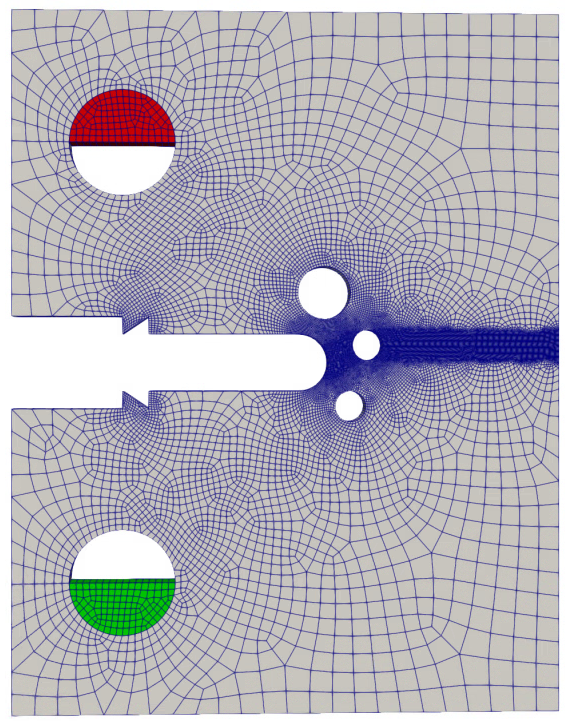
\includegraphics[width=0.4\textwidth]{results/pictures/frac_challenge/domain.png}
    \caption{Domain for fracture challenge}\label{fig:challenge_domain}
\end{figure}

% Top reaction force vs. loading-pin displacement u_y = 8*time (mm), with and without RaM.
% The x range stops at the end of the last RaM segment (_6.csv, t = 0.35625 -> u_y = 2.85 mm).
% RaM segments _1 to _6 start with an all-zero row at the restart time, so that row is dropped.
\pgfplotsset{
    fcskipfirst/.style={x filter/.expression={\coordindex==0 ? nan : x}},
}
\begin{figure}[htbp]
    \centering
    \begin{tikzpicture}
        \begin{axis}[
                width=0.6\textwidth,
                height=0.4\textwidth,
                xmin=0, xmax=2.85,
                restrict x to domain=0:2.85,
                xlabel={Loading pin displacement $u_y$ (\unit{\milli\meter})},
                ylabel={Top reaction force},
                legend pos=north east,
                legend cell align=left,
                grid=major,
            ]
            \addplot[blue, line width=1.6pt] table[col sep=comma, x expr=8*\thisrow{time}, y=reaction_top] {results/data/frac_challenge/frac_challenge_1e4meshnotch_single_0.csv};
            \addlegendentry{No RaM}
            \addplot[red, line width=0.8pt] table[col sep=comma, x expr=8*\thisrow{time}, y=reaction_top] {results/data/frac_challenge/frac_challenge_meshnotch_1e4_0.csv};
            \addlegendentry{RaM}
            \foreach \i in {1,...,6} {
                    \addplot[red, line width=0.8pt, fcskipfirst, forget plot] table[col sep=comma, x expr=8*\thisrow{time}, y=reaction_top] {results/data/frac_challenge/frac_challenge_meshnotch_1e4_\i.csv};
                }
        \end{axis}
    \end{tikzpicture}
    \caption{Top reaction force vs.\ loading pin displacement with and without RaM.}\label{fig:challenge_reaction}
    \label{fig:sfc_reactiondisp}
\end{figure}


\FloatBarrier{}



\subsection{Tophat}\label{ss:tophat}

\subsection{Torsion}\label{ss:torsion}
